\lhead{Capítulo \ref{ch_2}}
%\rhead{\newtitle}
\rhead{}
\cfoot{\thepage}
\renewcommand{\headrulewidth}{1pt}
\renewcommand{\footrulewidth}{1pt}

\chapter{Adaptación al Sitio}\label{ch_2}
%\noindent Aquí se escribe el segundo capítulo de la tesis


Existen diferentes enunciados a los que se hace referencia mediante el término Adaptación al Sitio (SA  por sus siglas en ingles).\\

\enquote{\textit{todos los métodos estadísticos desarrollados para reducir la incertidumbre en el recurso solar local que buscan mejorar los datos de irradiancia derivados de satélites (disminuyendo sus errores aleatorios y, sobre todo, su sesgo) utilizando características de observaciones terrestres correspondientes durante períodos de tiempo superpuestos}}\citep{POLO2016}.


\enquote{\textit{los procedimientos para corregir errores sistemáticos en un período prolongado de datos modelados en cuadrícula, utilizando un período corto de mediciones terrestres como referencia objetiva}}\citep{YANG2021427}. 

\enquote{\textit{la aplicación de un método de corrección a productos DSR en cuadrícula mediante el uso de mediciones del sitio}} \citep{rs17101720}.\\


Aunque cada definición tiene un matiz distinto, todas coinciden en lo esencial: ajustar los datos de irradiancia solar obtenidos por satélite o modelos para que representen con mayor precisión las condiciones reales de un sitio específico.\\ 

Una interpretación de estas definiciones nos permite expresar que este proceso consiste en aplicar correcciones estadísticas a los datos de radiación solar obtenidos de satélites o modelos numéricos (como los re-análisis), con el fin de hacerlos más representativos del sitio específico donde se quiere aplicar —por ejemplo, una futura planta solar.\\




\begin{figure}
    \centering
    \includegraphics[width=0.97\linewidth]{figuras/SiteAdapation-Example.png}
    \caption{Comparación de irradiancia solar diaria entre datos de satélite sin adaptar, datos de satélite adaptados y mediciones locales en el sitio de referencia. Se observa cómo la adaptación al sitio corrige el sesgo sistemático y mejora la representatividad de los datos satelitales.}
    \label{fig:example}
\end{figure}


Dado que los datos modelados tienen errores, especialmente errores sistemáticos (sesgos) y errores aleatorios, esta técnica usa mediciones reales de radiación tomadas en el sitio (aunque sea durante un período corto) como referencia para calibrar los datos. El objetivo es reducir la incertidumbre y mejorar la precisión en las estimaciones de largo plazo.\\

La Figura \ref{fig:example}  ilustra una comparación entre tres conjuntos de datos de irradiancia solar a lo largo de un mes:

Medición en sitio (línea sólida): representa la referencia real tomada con instrumentos locales.

Satélite sin adaptar (línea discontinua): se observa un sesgo, ya que la serie está sistemáticamente desplazada respecto a la referencia. Además, los picos y valles no coinciden con exactitud, reflejando errores aleatorios.

Satélite adaptado (línea punteada): tras aplicar el procedimiento de adaptación al sitio, la serie corregida se ajusta mucho mejor a la referencia. El sesgo desaparece en gran medida y la forma de la curva sigue más de cerca la variabilidad de las mediciones locales.

Puede verse cómo la adaptación al sitio reduce tanto el error sistemático como la dispersión, logrando que los datos derivados de satélite sean más representativos de las condiciones reales de irradiancia en el lugar de interés.\\


\begin{figure}
    \centering
    \includegraphics[width=0.97\linewidth]{figuras/siteAdaptation.png}
    \caption{Adaptación al Sitio sobre una serie genérica}
    \label{fig:site-adapation}
\end{figure}

En la Figura \ref{fig:site-adapation} puede verse el resultado que busca obtenerse al aplicar una adaptación al sitio. En color naranja se muestra la serie de medidas en tierra y en color azul la serie modelada, ambos casos con estilo de linea lleno. Debe tenerse en cuenta que el fondo cambiante de color (blanco y salmón) está realizado así a propósito.\\ 

Vamos a presentar una pequeña analogía que ayude a explicar de manera más cotidiana la idea general del preceso de SA.
\begin{quote}
Pensemos en que tienes un \textbf{termómetro económico} en tu casa (equivalente a los datos de un \textit{modelo}), 
pero al lado colocas uno profesional del hospital (equivalente a la \textit{medición en sitio}).  

Al comparar, notas que tu termómetro casero siempre marca \(-2\,^{\circ}\mathrm{C}\) respecto al valor real.  

Si corriges ese error sumando esos 2 grados, tu termómetro económico comienza a ser \textbf{útil y confiable} para el uso diario.  

\medskip
$\Rightarrow$ Eso es, en esencia, la \textbf{adaptación al sitio}: reducir el error de un modelo a partir de  una referencia local.
\end{quote}



\begin{figure}[H]
\centering
\includegraphics[width=\textwidth]{figuras/scatter-01.png}
\caption{Diagrama de dispersión entre mediciones en sitio y estimaciones satelitales.
Antes de la adaptación (puntos rojos), los datos muestran un sesgo claro al situarse por debajo de la línea 1:1. 
Después de la adaptación (puntos verdes), las estimaciones se alinean mucho mejor con la referencia, reduciendo el error sistemático.}
\label{fig:scatter01}
\end{figure}



La Figura \ref{fig:scatter01} muestra de manera evidente el efecto de la adaptación al sitio:

Antes de la corrección (rojo): los puntos están sistemáticamente alejados de la línea 1:1, lo que indica que el satélite subestima los valores reales de irradiancia. Existe un sesgo claro.

Después de la corrección (verde): los puntos se agrupan alrededor de la línea 1:1, lo que significa que las estimaciones satelitales ahora representan con mayor fidelidad las mediciones en sitio.




\section{Historia}
Uno de los principales aportes sobre el tema fue realizado en el trabajo de \cite{POLO2016} en el marco de la Tarea 46 del Programa de Calefacción y Refrigeración Solar de la Agencia Internacional de la Energía Evaluación y pronóstico de recursos solares. En este trabajo se indica que la idea general de este proceso de corrección o calibración de datos modelados es similar a lo que se ha desarrollado en  la industria eólica en el pasado \citep{Potter}.
 
Según Polo y sus colaboraores AS en un término actualmente utilizado en proyectos de energía solar para referirse a la mejora que puede lograrse en la irradiancia solar derivada de satélite y los datos del modelo cuando se utilizan mediciones terrestres locales a corto plazo para corregir errores sistemáticos y sesgos en el conjunto de datos original. A partir de esta idea general se han agrupado a los diversos métodos para SA en cinco categorías en las cuales se comprenden las principales estrategias para mejorar la precisión y reducir la incertidumbre en las estimaciones de radiación solar derivadas de satélites mediante el uso de mediciones locales de corta duración.

\begin{enumerate}
    \item Métodos basados en modelos físicos (Physically based methods)\\
        Ajustan los datos de entrada atmosféricos (como la turbidez por aerosoles o el vapor de agua) para que los resultados coincidan mejor con las observaciones en tierra. Ejemplos: uso del modelo REST2 y corrección del AOD (Aerosol Optical Depth)
    \item Métodos estadísticos (Statistical methods) \\
        Ajustan los datos del modelo para eliminar errores sistemáticos (sesgo) y mejorar la concordancia con datos medidos localmente.

        \begin{itemize}
            \item Eliminación de sesgo mediante adaptación lineal
            \item Métodos no lineales (transformación de características, polinomios, etc.)
            \item MOS (Model Output Statistics)
            \item MCP (Measure–Correlate–Predict)
            \item Adaptación regional (usando estaciones cercanas)
            \item Adaptación usando funciones de distribución acumulativa (CDF)
        \end{itemize}
        
    \item Adaptación de parámetros de entrada del modelo satelital \\
        Se modifican directamente los parámetros de entrada del modelo (como el índice de claridad o datos atmosféricos) en lugar de los resultados de irradiancia.
    \item Técnicas MCP aplicadas a datos satelitales y de reanálisis \\
        Uso de métodos de correlación-predicción (común en energía eólica) para extender los datos de corto plazo a largo plazo con apoyo en modelos de reanálisis.
        
    \item Combinación de datos satelitales con modelos meteorológicos numéricos (NWP)\\
        Mejora de la precisión mediante regresiones no paramétricas (como modelos aditivos generalizados - GAM) que combinan datos satelitales con modelos meteorológicos.
\end{enumerate}


Además de presentar la clasificación anterior, se han indicado algunas directrizces que deben ser tomadas en cuenta en un proceso de adaptación. \\



A partir del año 2020 se comenzaron a publicar diversos trabajos sobre Adaptación al Sitio (SA). En \citep{POLO2020} se presentan los resultados de adaptaciones realizadas en diez estaciones a escala horaria, considerando ocho modelos satelitales y dos de re-análisis. En \citep{Fernández2020} se evaluaron los resultados de la adaptación al sitio utilizando regresiones lineales múltiples (MLR) y se combinaron estos resultados con un ajuste mediante mapeo de cuantiles (QM). Este enfoque de ensamble de modelos mostró una reducción promedio del 1,7\% en el sesgo relativo y del 3,3\% en la desviación cuadrática media relativa a escala horaria. El estudio también sugiere que un año de datos es suficiente para entrenar los modelos de ajuste.

En el trabajo de \citep{BABAR2020} se evaluó el desempeño de la SA en los valores medios diarios del modelo satelital CLARA-A2 y del modelo de re-análisis ERA5. Para ello, se utilizó un modelo de Random Forest para la regresión, incorporando como predictores los valores de GHI modelados por CLARA-A2 y ERA5, sus respectivos índices de cielo despejado y el ángulo cenital solar medio. Los resultados demostraron una reducción de la desviación cuadrática media de 17,9 W/m² a 16,2 W/m² y una corrección completa del sesgo inicial de -1,5 W/m². La motivación para adoptar un modelo de regresión basado en aprendizaje automático surgió de la hipótesis de que este tipo de algoritmo podría aplicar funciones de regresión distintas a cada subconjunto del espacio de datos predictivos. Este trabajo es uno de los primeros en utilizar modelos de aprendizaje automático como Random Forest para determinar una función de ajuste que calibra las mediciones en tierra y puede aplicarse a series de largo plazo.

A partir del trabajo de Babar y colaboradores, se han publicado diversos estudios en los que se exploran modelos de aprendizaje automático como alternativa para determinar funciones de ajuste sobre series modeladas, ya sean satelitales o de re-análisis.

En \citep{NARVAEZ2021} se evaluó la adaptación al sitio en series horarias, explorando el uso de redes neuronales y los modelos Random Forest y AdaBoost. El rendimiento de estos modelos se evaluó en función de las métricas obtenidas en comparación con los ajustes realizados mediante QM y MLR, donde Random Forest logró una mejora aproximada del 38\% con respecto a QM y MLR.

En \citep{YANG2021} se presenta una alternativa denominada Adaptación al Sitio Probabilística, que aprovecha la disponibilidad de múltiples modelos de estimación simultáneamente. Este enfoque combina regresiones de cuantiles sobre múltiples modelos a la vez para mejorar la precisión de la adaptación al sitio.

En el trabajo de \citep{SALAMALIKIS2022}, se aplicó SA al modelo Heliosat-4 con una resolución horaria mediante el entrenamiento de diferentes modelos de regresión para condiciones de cielo despejado y nublado, considerando segmentos de datos basados en rangos de 15° del ángulo cenital solar. En este estudió se reportó  que el sesgo se redujo en un 50\% y la desviación cuadrática media disminuyó en un 3,8\% en comparación con las estimaciones sin SA. Los mejores resultados de este trabajo se obtuvieron utilizando modelos de regresión basados en árboles de decisión, en particular Random Forest. Además, una característica a destacar sobre este trabajo es que los autores han buscado eliminar la estacionalidad de la serie definiendo $\Delta_{GHI}$ como la diferencia entre la GHI medida y la GHI modelada. Esta variable se utiliza entonces como objetivo para los modelos de regresión, y la GHI adaptada se calcula como la suma del GHI modelada y $\Delta_{GHI}$. Puede considerarse que los autores en este trabajo han buscado quitar la \enquote{\textit{estacionalidad}} de la serie. Esta práctica es ampliamente conocida y estudiada en el área del análisis de series temporales, es recomendada y analizada en estudios como \citep{THORNTON2013, Claveria2015}.   


En \citep{ZAINALI2024} se evaluó un proceso de SA en tres sitios del norte de Europa utilizando diversos ajustes de mapeo de cuantiles y modelos de aprendizaje automático para ajustar los datos del modelo STRANG. Los hallazgos indican que los modelos de aprendizaje automático generalmente obtienen un rendimiento superior al de los métodos estadísticos, logrando una mejora de hasta el 9,2\% en la reducción del sesgo.


\section{Características}

Entendiendo que SA se define como el proceso de corrección de las series de irradiancia solar modeladas (ya sean satelitales o de reanálisis) mediante un periodo corto de mediciones terrestres de alta calidad. Entre sus principales características se destacan:

Objetivo principal: reducir sesgos sistemáticos y errores aleatorios en las estimaciones de irradiancia, mejorando su precisión y representatividad local \citep{POLO2020, Fernández2020}.

Dependencia del sitio: el desempeño de los métodos de adaptación es altamente dependiente de las condiciones locales de nubosidad, aerosoles y régimen de radiación; no existe un modelo universal válido para todas las regiones \citep{ZAINALI2024}.

Duración de las mediciones necesarias: se ha demostrado que series de aproximadamente un año de datos de medición in-situ suelen ser suficientes para entrenar y validar los modelos de ajuste \citep{POLO2020, ZAINALI2024}.

Diversidad metodológica: existen enfoques físicos, estadísticos y basados en aprendizaje automático (p. ej. Random Forest, redes neuronales), con desempeños variables según el contexto \citep{BABAR2020, NARVAEZ2021}.

Aplicabilidad en cualquier fuente de modelado y escala temporal: la SA puede aplicarse tanto a productos derivados de satélite como a bases de datos de reanálisis, así como a resoluciones horarias, diarias o mensuales, dependiendo de la aplicación energética \citep{Fernández2020, Quansah2024}.

Accesibilidad: en la práctica, se están desarrollando herramientas de libre acceso (p. ej. paquetes en R como SiteAdapt) que facilitan la implementación de los métodos de corrección \citep{Fernández2020}.


\section{Ventajas y Desventajas}

\subsection*{Ventajas}

Reducción significativa del sesgo: numerosos estudios han mostrado disminuciones de hasta el 100\% en el sesgo relativo de GHI tras la aplicación de SA \citep{BABAR2020,  SALAMALIKIS2022}.

Mejora en la precisión estadística: métricas como RMSE, desviación relativa y similitud de distribuciones mejoran de forma consistente (con reducciones del 3–10\% en RMSE en muchos casos) \citep{Fernández2020, ZAINALI2024}.

Mayor confiabilidad bancaria: la SA es una práctica solicitada por instituciones financieras en proyectos solares, al reducir la incertidumbre en los estudios de recurso \citep{Fernández2020}.

Flexibilidad metodológica: la posibilidad de usar métodos simples (regresión lineal) o complejos (machine learning) permite adaptar la técnica a distintos recursos de datos y niveles de complejidad \citep{NARVAEZ2021, YANG2021}.

Aplicaciones múltiples: útil para proyectos fotovoltaicos, termosolares y agrivoltaicos, ya que mejora la estimación de radiación tanto para dimensionamiento energético como para balances agrícolas \citep{ZAINALI2024}.

\subsection*{Desventajas}

Dependencia de datos locales: requiere campañas de medición en el sitio, que pueden ser costosas o inexistentes en ciertas regiones \citep{Quansah2024}.

Limitación espacial: la corrección es estrictamente local y no siempre extrapolable a regiones cercanas sin mediciones adicionales \citep{POLO2020}.

No generalización: los resultados dependen del modelo de origen y de las condiciones climáticas locales; un método que funciona bien en un sitio puede no ser adecuado en otro \citep{Fernández2020, ZAINALI2024}.

Sobrecoste computacional: en el caso de los métodos de aprendizaje automático, la calibración y validación pueden requerir recursos computacionales elevados y experiencia técnica.

Persistencia de incertidumbre: aunque se reduzca, nunca se elimina completamente la incertidumbre de la estimación; además, eventos extremos o fenómenos atmosféricos poco frecuentes pueden no quedar bien representados.





\section{Modelos de Aprendizaje Automático} \label{MLM}
Aunque Arthur Samuel no fue el primero en publicar un artículo que empleara el término "aprendizaje automático", se le atribuye la creación y definición de este concepto como el campo especializado que conocemos hoy. En su trabajo `Algunos estudios sobre aprendizaje automático usando el juego de damas' \cite{samuel1959}, presentó el aprendizaje automático como una rama de la informática que permite a las computadoras mejorar su desempeño sin necesidad de ser programadas de forma explícita.

Si bien la definición original de Samuel no lo menciona directamente, un aspecto fundamental del aprendizaje automático es el autoaprendizaje. Este concepto implica el uso de modelos estadísticos para identificar patrones y optimizar el rendimiento con base en datos e información empírica, sin requerir instrucciones de programación explícitas \cite{Theobald2024}.

Samuel no infirió que las máquinas puedan tomar decisiones sin programación previa. Al contrario, el aprendizaje automático depende en gran medida de la entrada de código. En cambio, observó que las máquinas pueden realizar una tarea específica utilizando datos de entrada en lugar de depender de un comando de entrada directo.

\begin{figure}[H]
    \centering
    \includegraphics[scale=0.5]{figuras/ML.pdf}
    \caption{Comparación entre el comando de entrada y los datos de entrada}
    \label{fig:ML}
\end{figure}



\subsection{Modelo de red neuronal}

No existe una definición única de lo que es una red neuronal artificial, pero distintas fuentes proponen descripciones complementarias. Algunas de las más comunes son:

\begin{itemize}
    \item Un modelo computacional, paralelo, compuesto por unidades procesadoras adaptativas altamente interconectadas.
    \item Un sistema de procesamiento de la información que aplica principios inspirados en la organización del cerebro humano.
    \item Un modelo matemático diseñado para emular, de manera simplificada, el funcionamiento del cerebro.
    \item Un sistema de información con características de funcionamiento similares a las redes neuronales biológicas.
    \item Una red adaptativa que combina técnicas de procesamiento paralelo de la información.
    \item Una extensión de los métodos clásicos estadísticos, especialmente útil en el reconocimiento de patrones.
\end{itemize}

En todas estas definiciones se aprecia un componente de \textit{simulación biológica}. Las redes neuronales artificiales se inspiran en el cerebro humano en el sentido de que el procesamiento de la información se distribuye entre elementos básicos llamados \textit{neuronas}. Estas están interconectadas mediante \textit{pesos sinápticos}, que se ajustan a lo largo del tiempo durante un proceso denominado \textit{aprendizaje}. En términos simples, aprender consiste en modificar la intensidad de las conexiones entre neuronas para resolver una tarea determinada.

\subsubsection*{Neurona artificial}

Los componentes básicos de una neurona artificial son:

\begin{enumerate}
    \item Un conjunto de conexiones ponderadas (pesos sinápticos).
    \item Un sesgo, que actúa como umbral de activación.
    \item Un sumador, que agrega las entradas multiplicadas por sus pesos correspondientes.
    \item Una función de activación no lineal, que permite ampliar la capacidad de representación del modelo.
\end{enumerate}

\begin{figure}[H]
    \centering
    \includegraphics[scale=0.7]{figuras/neurona.png}
    \caption{Esquema de una neurona artificial}
    \label{fig:neurona}
\end{figure}

El funcionamiento matemático de una neurona artificial puede expresarse como:

\begin{equation}
    salida = f(y) = f\left( \sum_{k=0}^{n} w_{k}x_{k} \right)
    \label{eq:neurona}
\end{equation}

donde $x_i$ son las entradas, $w_i$ los pesos sinápticos y $x_0=1$ corresponde al sesgo con coeficiente $w_0$. La función $f$ representa la activación de la neurona.

\subsubsection*{Funciones de activación}

Las funciones de activación más comunes se resumen en la Tabla \ref{tab:activations}. Estas permiten introducir no linealidad en el modelo, lo cual es fundamental para que la red pueda aproximar funciones complejas.

\begin{table}[h]
    \centering
    \renewcommand{\arraystretch}{1.5}
    \begin{tabular}{|>{\centering\arraybackslash}p{2cm}|>{\centering\arraybackslash}p{5cm}|>{\centering\arraybackslash}p{8cm}|}
        \hline
        \textbf{Función} & \textbf{Expresión} & \textbf{Comentario} \\ 
        \hline
        Signo & 
        \( f(x) =
        \begin{cases} 
            1, & \text{si } x \geq 0 \\ 
            -1, & \text{si } x < 0 
        \end{cases} \)  
        & Usada en los primeros modelos de neuronas artificiales. \\ 
        \hline
        Sigmoide & 
        \( f(x) = \frac{1}{1 + e^{-x}} \)  
        & Transición suave entre 0 y 1, útil en clasificación binaria. \\ 
        \hline
        Tangente hiperbólica & 
        \( f(x) = \frac{e^x - e^{-x}}{e^x + e^{-x}} \)  
        & Similar a la sigmoide, pero con valores entre -1 y 1. \\ 
        \hline
        ReLU & 
        \( f(x) = \max(0, x) \)  
        & Una de las más usadas actualmente; evita problemas de gradiente. \\ 
        \hline
        Softmax & 
        \( f(x_i) = \frac{e^{x_i}}{ \sum_{k} e^{x_k} } \)  
        & Utilizada en la salida de modelos de clasificación multiclase. \\ 
        \hline
    \end{tabular}
    \caption{Funciones de activación más comunes en redes neuronales artificiales.}
    \label{tab:activations}
\end{table}

\subsubsection*{Perceptrón y sus limitaciones}

El perceptrón simple, basado en esta estructura, funciona como un clasificador binario que sólo puede resolver problemas linealmente separables. El procedimiento de aprendizaje consiste en:

\begin{enumerate}
    \item Inicializar aleatoriamente los pesos $w_{k}$.
    \item Establecer el parámetro de aprendizaje $\alpha$.
    \item Calcular la salida: $salida = signo(\sum_{k=0}^{n} w_{k} x_{k})$.
    \item Calcular el error: $error = salida_{deseada} - salida$.
    \item Actualizar los pesos: $w_{k} = w_{k} + \alpha \cdot error \cdot x_{k}$.
    \item Repetir el proceso.
\end{enumerate}

Aunque este modelo es simple y útil, su capacidad de representación es limitada. Para superar estas restricciones se introducen las redes \textbf{multicapa}.

\subsubsection*{Perceptrón Multicapa (MLP)}

El \textit{Perceptrón Multicapa} (MLP, por sus siglas en inglés) organiza neuronas en diferentes capas: una capa de entrada, una o varias capas ocultas y una capa de salida (Fig. \ref{fig:MLP}). Gracias a esta estructura, el MLP puede aproximar funciones no lineales y resolver problemas más complejos.

\begin{figure}[H]
    \centering
    \includegraphics[scale=0.6]{figuras/MLP.png}
    \caption{Esquema de una red neuronal multicapa (MLP).}
    \label{fig:MLP}
\end{figure}

Un MLP con una capa oculta se puede definir como:

\begin{equation}
\hat{y} = f^{(2)}\Big( W^{(2)} \cdot f^{(1)}( W^{(1)} x + b^{(1)} ) + b^{(2)} \Big),
\end{equation}

donde $x$ es el vector de entrada, $W^{(1)}, W^{(2)}$ son matrices de pesos, $b^{(1)}, b^{(2)}$ los sesgos y $f^{(1)}, f^{(2)}$ las funciones de activación de cada capa \cite{ghanou2016mlp}.

\subsubsection*{MLP en la estimación de irradiancia solar}

En el contexto de la estimación de la irradiancia global horizontal (GHI), el MLP puede verse como un \textit{equipo de expertos neuronales}. Cada neurona aporta una “opinión parcial” a partir de las variables meteorológicas (nubosidad, humedad, ángulo solar, aerosoles), mientras que las capas ocultas integran estas opiniones para refinar la predicción de manera no lineal \cite{torobayona2012mlp}.  

\begin{figure} 
\centering 
\begin{tikzpicture}[node distance=2.2cm]
\tikzstyle{neuron} = [circle, draw, minimum size=1cm, fill=blue!20, text centered]
\tikzstyle{output} = [rectangle, draw, thick, rounded corners, text centered, minimum height=1cm, minimum width=3cm, fill=green!20]

\node (input1) [neuron] {Nubosidad};
\node (input2) [neuron, below of=input1] {Humedad};
\node (input3) [neuron, below of=input2] {Ángulo solar};

\node (hidden1) [neuron, right of=input1, xshift=4cm] {Oculta 1};
\node (hidden2) [neuron, below of=hidden1] {Oculta 2};

\node (final) [output, right of=hidden1, xshift=4cm, yshift=-1cm] {Predicción de GHI};

\foreach \i in {input1,input2,input3}{
\foreach \j in {hidden1,hidden2}{
\draw[flecha] (\i.east) -- (\j.west);
}
}
\foreach \j in {hidden1,hidden2}{
\draw[flecha] (\j.east) -- (final.west);
}
\end{tikzpicture}
\caption{Analogía del MLP como un conjunto de expertos neuronales que refinan la predicción de la GHI.}
\label{fig:mlp_experts}
\end{figure}

El MLP ofrece una estructura potente y flexible capaz de modelar relaciones no lineales complejas, esto permite considerarlo como una herramienta adecuada para la estimación de irradiancia solar.

\subsubsection*{Ejemplo práctico de entrenamiento en un MLP}

Para ilustrar el funcionamiento del \textit{Perceptrón Multicapa} (MLP), consideremos un ejemplo sencillo con dos entradas, una capa oculta con dos neuronas y una salida (Figura \ref{fig:mlp_ejemplo}).  

\begin{figure}[H]
    \centering
    \includegraphics[scale=0.2]{figuras/mlp.png}
    \caption{Ejemplo de un MLP con dos entradas, dos neuronas ocultas y una salida.}
    \label{fig:mlp_ejemplo}
\end{figure}





El cálculo de las salidas se realiza en dos fases: propagación hacia adelante (\textit{forward pass}) y retropropagación del error (\textit{backpropagation}).

\paragraph{1. Propagación hacia adelante}
Las entradas $x_1$ y $x_2$ llegan a las dos neuronas ocultas $a$ y $b$:

\begin{equation}
    y_{a} = w_{0a} + w_{1a}x_{1} + w_{2a}x_{2}, \quad O_{a} = f(y_{a})
\end{equation}
\begin{equation}
    y_{b} = w_{0b} + w_{1b}x_{1} + w_{2b}x_{2}, \quad O_{b} = f(y_{b})
\end{equation}

Las salidas $O_{a}$ y $O_{b}$ alimentan a la neurona de salida $c$:

\begin{equation}
    y_{c} = w_{0c} + w_{ac}O_{a} + w_{bc}O_{b}, \quad \hat{y} = f(y_{c})
\end{equation}

donde $f(\cdot)$ es una función de activación diferenciable (sigmoide, tangente hiperbólica, ReLU, etc.).

\paragraph{2. Cálculo del error}
Dado un valor deseado $y$, el error cuadrático medio (ECM) para un ejemplo es:

\begin{equation}
    E = \frac{1}{2}(y - \hat{y})^2
\end{equation}

\paragraph{3. Retropropagación}
El objetivo es calcular cómo varía el error respecto a cada peso y ajustar estos valores en la dirección del gradiente descendente.

\begin{itemize}
    \item Para la salida $c$:
    \begin{equation}
        \delta_c = (y - \hat{y}) f'(y_{c})
    \end{equation}
    \item Para las neuronas ocultas $a$ y $b$:
    \begin{equation}
        \delta_a = f'(y_{a}) \cdot (w_{ac}\delta_c), \quad
        \delta_b = f'(y_{b}) \cdot (w_{bc}\delta_c)
    \end{equation}
\end{itemize}

\paragraph{4. Actualización de pesos}
Finalmente, los pesos se actualizan usando una tasa de aprendizaje $\eta$:

\begin{equation}
    w_{ij} \leftarrow w_{ij} + \eta \cdot \delta_j \cdot x_i
\end{equation}

donde $x_i$ es la entrada a la neurona $j$. Este procedimiento se repite para todos los ejemplos del conjunto de entrenamiento hasta que el error sea lo suficientemente pequeño.

\paragraph{5. Resumen del ciclo de aprendizaje}
\begin{enumerate}
    \item Inicializar pesos y sesgos aleatoriamente.
    \item Realizar la propagación hacia adelante para obtener la salida $\hat{y}$.
    \item Calcular el error $E$ comparando con el valor real $y$.
    \item Retropropagar el error para obtener los deltas $\delta$ de cada neurona.
    \item Actualizar los pesos usando la regla de gradiente descendente.
    \item Repetir el proceso hasta la convergencia.
\end{enumerate}

Este procedimiento es la base del entrenamiento de redes neuronales modernas. A pesar de su simplicidad, este esquema permite que los MLP aproximen relaciones altamente no lineales, siendo especialmente útiles para la estimación de la irradiancia solar, donde influyen múltiples variables meteorológicas de manera simultánea.













\subsection{Arboles de Decisión}
Los árboles de decisión son modelos no paramétricos (es decir que no se no toman suposiciones previas sobre la forma de distribución de los datos) que se utilizan principalmente para la resolución de problemas de clasificación o regresión. También son conocidos como árboles de clasificación y regresión (CART, classification and regression trees). Este tipo de modelo fue propuesto por Leo Breiman en el libro \cite{breiman1984}

Los árboles de decisión se basan en una serie de reglas de decisión para dividir el espacio de características predictoras en un número menor de regiones disjuntas en cada una de las cuales los valores de la variable respuesta son similares.

Un árbol de decisión parte del conjunto de datos de entrenamiento, correspondiente a un nodo raíz, y lo va dividiendo recursivamente en subconjuntos de datos homogéneos, dando lugar a nuevos nodos. La manera de formar los subgrupos es mediante la formulación de preguntas con respuesta binaria (si la variable respuesta es `jugar al tenis' se formula la pregunta ¿Sí o No juega al tenis?; si es `pesa más o menos de 75 kg.' la pregunta es ¿el peso es <=75 o >75?). \\

Los árboles de decisión se pueden clasificar en función del tipo de variable respuesta, si la variable de respuesta $y$ es cuantitativa el árbol es de regresión, si $y$ es cuantitativa el árbol es de clasificación.

\begin{figure}
    \centering
    \includegraphics[width=0.25\linewidth]{figuras/tree_1.png}
    \caption{Ejemplo Árbol de Regresión. Para los datos de Hitters, se construye un árbol de regresión para predecir el logaritmo del salario de un jugador de béisbol, en función del número de años que ha jugado en las grandes ligas y el número de hits que realizó en el año anterior.}
    \label{fig:tree}
\end{figure}


El proceso general de construcción de un árbol de regresión puede describirse en dos pasos:
\begin{enumerate}
    \item  Dividir el espacio de predictores: es decir, el conjunto de valores posibles de $X_1, X_2, ..., X_p$ se divide en $J$ regiones distintas y no superpuestas, $R_1, R_2,..,R_J$.

    \item Hacer una predicción para cada región: para cada observación que cae en una región $R_j$, la predicción será simplemente la media de los valores de respuesta de las observaciones de entrenamiento dentro de $R_j$.
\end{enumerate}


\subsection{Random Forest}
\addcontentsline{toc}{subsection}{Random Forest: Un Enfoque de Aprendizaje Autom\'atico}

El algoritmo \textbf{Random Forest} (RF) es un modelo de aprendizaje supervisado de tipo \textit{ensemble} que se utiliza para resolver problemas de \textbf{clasificaci\'on} y \textbf{regresi\'on} \cite{louppe2015, salman2024}. Este m\'etodo, conceptualizado por Leo Breiman, es una extensi\'on del concepto de \textit{bagging} y se ha establecido como una t\'ecnica muy precisa y robusta en la miner\'ia de datos \cite{cutler2011}.


El fundamento de RF es la construcci\'on de un conjunto de m\'ultiples \'arboles de decisi\'on, donde cada \'arbol se entrena sobre un subconjunto de datos generado de forma aleatoria \cite{salman2024}. La aleatoriedad se introduce en dos niveles principales para garantizar que los \'arboles sean diversos y que el modelo no se sobreajuste:

\begin{enumerate}
    \item \textbf{Muestreo con reemplazo (Bootstrapping)}: Se generan m\'ultiples submuestras del conjunto de datos de entrenamiento original, con la posibilidad de que una misma observaci\'on aparezca varias veces en la misma submuestra. Cada submuestra se usa para entrenar un \'arbol de decisi\'on individual \cite{salman2024}.
    \item \textbf{Selecci\'on aleatoria de variables}: En cada nodo de un \'arbol, el algoritmo selecciona un subconjunto aleatorio de las variables predictoras disponibles. La mejor divisi\'on del nodo se determina a partir de este subconjunto reducido \cite{cutler2011, salman2024}. Esta t\'ecnica reduce la correlaci\'on entre los \'arboles y mejora la capacidad de generalizaci\'on del modelo \cite{cutler2011}.
\end{enumerate}


La divisi\'on \'optima en cada nodo del \'arbol se basa en la minimizaci\'on de una funci\'on de costo, que var\'ia seg\'un el tipo de problema.

Para problemas de \textbf{clasificaci\'on}, se utilizan medidas de impureza como el \textbf{\'indice Gini} o la \textbf{Entrop\'ia}. El \'Indice Gini mide la probabilidad de que una muestra elegida al azar de un nodo sea clasificada err\'oneamente, y se calcula de la siguiente manera:
$$
I_G(p) = 1 - \sum_{i=1}^{c} p_i^2
$$
donde $c$ es el n\'umero de clases y $p_i$ es la proporci\'on de muestras de la clase $i$ en el nodo.

Para problemas de \textbf{regresi\'on}, el criterio de divisi\'on se basa en la minimizaci\'on de la varianza o el \textbf{Error Cuadr\'atico Medio (MSE)} de las predicciones en los nodos hijos:
$$
MSE = \frac{1}{n} \sum_{i=1}^{n} (y_i - \hat{y}_i)^2
$$
donde $n$ es el n\'umero de muestras, $y_i$ es el valor real y $\hat{y}_i$ es el valor predicho.

Para realizar una predicci\'on final, el algoritmo agrega los resultados de todos los \'arboles del \textit{bosque} \cite{salman2024}. En problemas de \textbf{clasificaci\'on}, la predicci\'on se basa en el \textbf{voto mayoritario} de los \'arboles. Para problemas de \textbf{regresi\'on}, la predicci\'on final es el promedio de los resultados de cada \'arbol individual:
$$
\hat{y}_{RF}(\mathbf{x}) = \frac{1}{B} \sum_{b=1}^{B} h_b(\mathbf{x})
$$
donde $B$ es el n\'umero total de \'arboles en el bosque y $h_b(\mathbf{x})$ es la predicci\'on del $b$-\'esimo \'arbol.


Random Forest ofrece varias ventajas significativas para el an\'alisis de datos \cite{cutler2011}:

\begin{itemize}
    \item \textbf{Resistencia al sobreajuste (\textit{overfitting})}: El algoritmo es intr\'insecamente resistente al sobreajuste, ya que el conjunto de \'arboles se entrena en subconjuntos aleatorios de datos \cite{salman2024}.
    \item \textbf{Manejo de variables}: Es capaz de manejar eficientemente un gran n\'umero de variables, incluso cuando hay valores perdidos, sin necesidad de imputaci\'on previa \cite{cutler2011}.
    \item \textbf{Estimaci\'on de la importancia de las variables}: El algoritmo proporciona una medida integrada que indica la contribuci\'on relativa de cada variable al modelo, lo que facilita la interpretaci\'on de los resultados \cite{cutler2011}.
\end{itemize}



\subsection{XGBoost}

El algoritmo \textit{Extreme Gradient Boosting} (XGBoost) es una implementación optimizada del método de \textit{Gradient Boosted Decision Trees} (GBDT) \cite{chen2016xgboost}.
Su funcionamiento consiste en combinar múltiples árboles de decisión simples para construir un modelo robusto, de manera semejante a cómo un equipo de especialistas aporta su conocimiento colectivo para tomar mejores decisiones.
XGBoost se ha consolidado como estado del arte en aprendizaje automático debido a su alto desempeño en tareas de clasificación y regresión en diversos dominios \cite{espinoza2020aplicacion}.\\


Para entender el algoritmo y su aplicación en la estimación de la GHI, podemos usar una analogía. Supongamos que deseamos predecir la GHI en un lugar específico.

Un único árbol de decisión actúa como un \textit{experto solitario}, que utiliza reglas simples para emitir un juicio, por ejemplo: \`si la nubosidad es alta, entonces la irradiancia será baja''. Aunque este razonamiento es útil, tiene limitaciones: la irradiancia también depende de la altura solar, aerosoles, humedad relativa o estacionalidad. Por ello, un solo árbol puede fallar al no capturar la complejidad completa del fenómeno.

XGBoost supera esta limitación mediante un \textit{comité de expertos}, es decir, un conjunto de árboles que se construyen secuencialmente para aprender de los errores de sus predecesores. Cada árbol nuevo se centra en corregir las predicciones incorrectas de los anteriores, especializándose en las regiones donde estos fallaron. Así, el modelo colectivo refina sus predicciones de manera progresiva. Esta dinámica se ilustra en la Figura \ref{fig:xgb_experts}.

Podemos compararlo con un proceso de deliberación científica: el primer investigador propone un modelo básico; otro detecta que no captura los días parcialmente nublados y lo corrige; un tercero ajusta los errores en días despejados con baja humedad. Con el tiempo, el grupo obtiene un modelo más completo que cualquiera de los expertos individuales.\\

Esta idea refleja la esencia del \textit{gradient boosting}: aprendizaje aditivo y secuencial, donde cada árbol se incorpora para reducir la pérdida residual del conjunto previo \cite{chen2016xgboost}. La fuerza del modelo final no está en la exactitud de cada árbol individual (clasificador débil), sino en la sinergia de todos ellos, formando un predictor colectivo altamente robusto.
En el caso de la estimación de GHI, el ensamble de árboles de XGBoost permite capturar relaciones complejas entre variables meteorológicas y solares, mientras controla el sobreajuste mediante regularización y técnicas adicionales como \textit{shrinkage} y submuestreo \cite{xgboostdoc}.

En resumen, si un árbol es un experto solitario con visión parcial, XGBoost funciona como un \textit{panel de expertos} que deliberan y corrigen mutuamente sus errores para alcanzar predicciones más precisas.

\begin{figure} \centering \begin{tikzpicture}[node distance=2.2cm] % Estilos de nodos
\tikzstyle{expert} = [rectangle, draw, rounded corners, text centered, text width=3.5cm, minimum height=1cm, fill=blue!15] \tikzstyle{consensus} = [rectangle, draw, thick, rounded corners, text centered, text width=4.5cm, minimum height=1.2cm, fill=green!20] % Nodos de expertos 
\node (exp1) [expert] {Árbol 1:\\ Si nubosidad alta $\Rightarrow$ baja irradiancia''}; \node (exp2) [expert, below of=exp1] {Árbol 2:\\ Corrige error en días despejados}; \node (exp3) [expert, below of=exp2] {Árbol 3:\\ Ajusta casos con alta humedad}; \node (exp4) [expert, below of=exp3] {Árbol 4:\\ Mejora predicción en invierno}; % Nodo de consenso 
\node (final) [consensus, right of=exp2, xshift=8cm, yshift=-1cm] {Consenso del Comité (XGBoost):\\ Predicción refinada de GHI}; % Flechas de cada experto al consenso 
% Definir un estilo para las flechas \usetikzlibrary{decorations.markings} 
% cargar librería 
\tikzset{ flecha/.style={ thick, postaction={decorate, decoration={ markings, mark=at position 1 with {\arrow{>}} }} } } 
% Dibujar las flechas para los nodos exp1, exp2, exp3, exp4 hacia final
\foreach \i in {1,2,3,4}{ \draw[flecha] (exp\i.east) -- +(2,0) |- (final.west); } \end{tikzpicture} \caption{Analogía del comité de expertos en XGBoost: cada árbol corrige los errores de sus predecesores y contribuye a una predicción final más precisa de la GHI.} \label{fig:xgb_experts} \end{figure}

Formalmente, el modelo se define como:

\begin{equation}
\hat{y}_i = \sum_{k=1}^{K} f_k(x_i), \quad f_k \in \mathcal{F}, 
\end{equation}

donde cada $f_k$ es un árbol de regresión (\textit{CART}) y $\mathcal{F}$ es el espacio de todos los árboles posibles. La función objetivo combina el error de predicción y la complejidad del modelo:

\begin{equation}
\mathcal{L} = \sum_{i=1}^{n} l(y_i, \hat{y}_i) + \sum_{k=1}^{K} \Omega(f_k), 
\end{equation}

con regularización definida como:

\begin{equation} 
\Omega(f) = \gamma T + \frac{1}{2}\lambda \|w\|^2, 
\end{equation}

donde $T$ es el número de hojas, $w$ los pesos de cada hoja, $\gamma$ penaliza la complejidad del árbol y $\lambda$ regula la magnitud de los pesos \cite{chen2016xgboost}.


% Nuevo TikZ para árbol simple 
\begin{figure}[H] 
\centering 
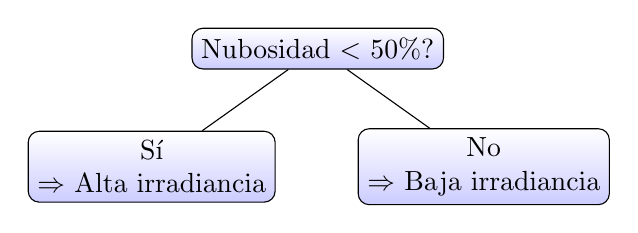
\begin{tikzpicture}[sibling distance=12em, every node/.style = {shape=rectangle, rounded corners, draw, align=center, top color=white, bottom color=blue!20}] 
\node {Nubosidad $<$ 50\%?} child { node {Sí \\ $\Rightarrow$ Alta irradiancia} } child { node {No \\ $\Rightarrow$ Baja irradiancia}};
\end{tikzpicture} 
\caption{Ejemplo de un árbol de decisión simple. XGBoost combina cientos de estos árboles débiles para construir un modelo poderoso.} 
\label{fig:treeexample} 
\end{figure}

XGBoost entrena los árboles de manera \textit{aditiva}, es decir, cada iteración añade un árbol que corrige los errores acumulados. Para ello utiliza una expansión de segundo orden de la función objetivo:

\begin{equation} 
\mathcal{L}^{(t)} \approx \sum_{i=1}^n \left[ g_i f_t(x_i) + \frac{1}{2} h_i f_t^2(x_i) \right] + \Omega(f_t), 
\end{equation}

donde $g_i$ y $h_i$ son el gradiente y la segunda derivada de la función de pérdida en la predicción previa. Esta formulación otorga estabilidad y precisión al proceso de entrenamiento \cite{chen2016xgboost}.


El proceso iterativo se representa en la Figura \ref{fig:boosting}.

% TikZ proceso iterativo 
\begin{figure}[H] 
\centering 
\begin{tikzpicture}[node distance=2cm] % Nodos de iteración 
\node[rectangle, draw, fill=blue!20, rounded corners, minimum width=3cm, minimum height=1cm] (tree1) {Árbol 1: predicción inicial}; \node[rectangle, draw, fill=blue!20, rounded corners, minimum width=3cm, minimum height=1cm, below of=tree1] (tree2) {Árbol 2: corrige errores del árbol 1}; \node[rectangle, draw, fill=blue!20, rounded corners, minimum width=3cm, minimum height=1cm, below of=tree2] (tree3) {Árbol 3: corrige errores acumulados}; % Nodo de modelo final 
\node[rectangle, draw, fill=green!20, rounded corners, minimum width=4cm, minimum height=1cm, right of=tree2, xshift=6cm] (finalmodel) {Modelo XGBoost final}; 
% Flechas 
\foreach \i/\j in {tree1/finalmodel, tree2/finalmodel, tree3/finalmodel}{ \draw[flecha] (\i.east) -- (\j.west); } 
\end{tikzpicture} 
\caption{Proceso iterativo: cada nuevo árbol corrige los errores del modelo acumulado.} 
\label{fig:boosting} 
\end{figure}


XGBoost también incluye estrategias adicionales para mejorar la generalización \cite{xgboostdoc}:

\begin{itemize} 
\item \textbf{Shrinkage ($\eta$):} funciona como una `moderación'' en las decisiones del comité, reduciendo el impacto de cada nuevo árbol. 
\item \textbf{Submuestreo:} cada árbol se entrena con una muestra parcial de datos y características, como consultar a un subgrupo de expertos para ganar diversidad en las opiniones. 
\item \textbf{Regularización adicional:} actúa como una \textit{disciplina} que limita la complejidad de cada experto, evitando que se vuelva demasiado específico. 
\end{itemize}

En este estudio se utilizó la librería \texttt{xgboost} \cite{xgboostdoc}, con soporte para paralelización y GPU, lo que permitió un entrenamiento eficiente incluso con grandes volúmenes de datos. Los principales hiperparámetros (\texttt{max\_depth}, \texttt{eta}, \texttt{n\_rounds}, $\lambda$, $\gamma$) se ajustaron mediante \textit{grid search}.

De acuerdo a las especificaciones teóricas presentadas, consideramos que el uso de XGBoost es especialmente adecuado para el análisis de irradiancia solar porque:

\begin{enumerate}
\item Captura relaciones no lineales entre variables atmosféricas y solares.
\item Reduce el sobreajuste mediante mecanismos internos de regularización.
\item Permite escalabilidad y eficiencia en grandes bases de datos.
\item Suele superar a otros ensambles como Random Forest \cite{espinoza2020aplicacion}.
\end{enumerate}

% TikZ esquema conceptual 
\begin{figure}[H] 
\centering 
\begin{tikzpicture}[node distance=1.5cm] \node[rectangle, draw, fill=blue!20, rounded corners, minimum width=3cm, minimum height=0.8cm] (t1) {Árbol 1}; \node[rectangle, draw, fill=blue!20, rounded corners, minimum width=3cm, minimum height=0.8cm, below of=t1] (t2) {Árbol 2}; \node[rectangle, draw, fill=blue!20, rounded corners, minimum width=3cm, minimum height=0.8cm, below of=t2] (t3) {Árbol 3}; \node[rectangle, draw, fill=green!20, rounded corners, minimum width=4cm, minimum height=1cm, right of=t2, xshift=6cm] (final) {Predicción colectiva XGBoost}; \foreach \i in {t1,t2,t3}{ \draw[flecha] (\i.east) -- +(2,0) |- (final.west); } \end{tikzpicture} \caption{Esquema conceptual: múltiples árboles (\textit{expertos}) corrigen iterativamente sus errores para formar un modelo robusto.} \label{fig:esquemaxgb} \end{figure}


La Figura \ref{fig:esquemaxgb} resumen la idea para una predicción generica utilizando XGBoost como modelo regresor.


En resumen, mientras que un árbol de decisión actúa como un experto solitario y XGBoost combina múltiples árboles secuencialmente, un MLP funciona como un sistema de neuronas interconectadas que colectivamente aprenden patrones complejos en los datos, logrando predicciones precisas de irradiancia solar.



\section{Entrenamiento y Prueba}

El proceso de construcción de un modelo de aprendizaje automático no termina en su diseño, sino que requiere fases diferenciadas de \textbf{entrenamiento}, \textbf{validación} y \textbf{prueba}, cuyo objetivo principal es garantizar la capacidad de generalización del modelo ante datos no observados.

\subsection*{División del conjunto de datos}
La práctica estándar consiste en dividir el conjunto de datos en tres subconjuntos:

\begin{itemize}
\item \textbf{Entrenamiento}: utilizado para ajustar los parámetros internos del modelo (pesos y sesgos en redes neuronales, divisiones en árboles de decisión, etc.).
\item \textbf{Validación}: empleado durante el entrenamiento para seleccionar hiperparámetros y evitar el sobreajuste (\textit{overfitting}). Una proporción habitual es 80\% para entrenamiento y 20\% para validación dentro del subconjunto inicial de entrenamiento \cite{Olivas2022}.
\item \textbf{Prueba (test)}: reservado exclusivamente para la evaluación final. Nunca se utiliza en la fase de ajuste, ya que su propósito es ofrecer una estimación imparcial del error de generalización \cite{Mostafa2012}.
\end{itemize}

\subsection*{Dinámica de entrenamiento}
Durante el entrenamiento, el error de entrenamiento disminuye progresivamente a medida que el modelo se ajusta a los datos. Paralelamente, el error de validación suele descender inicialmente, reflejando la mejora de la capacidad de generalización, hasta que alcanza un punto mínimo. A partir de ahí, si el entrenamiento continúa, el error de validación aumenta, lo que indica que el modelo comienza a memorizar los datos y pierde capacidad predictiva. Este fenómeno se conoce como \textbf{sobreajuste}, y la estrategia recomendada es detener el entrenamiento en el punto donde el error de validación es mínimo, aplicando técnicas como \textit{early stopping} o el almacenamiento de los mejores pesos (\textit{model checkpointing}) \cite{Olivas2022}.



\begin{figure}[H]
    \centering
    \includegraphics[scale=0.6]{figuras/dinamicatv.png}
    \caption{Dinámica de entrenamiento de un modelo de aprendizaje automático. La curva azul muestra el error de entrenamiento, que disminuye progresivamente a medida que el modelo se ajusta a los datos. La curva naranja representa el error de validación, que disminuye inicialmente reflejando la mejora de la capacidad de generalización, pero comienza a aumentar después de la mejor época (línea roja discontinua), evidenciando el sobreajuste.}
    \label{fig:dinamica}
\end{figure}


La figura \ref{fig:dinamica} ilustra la dinámica durante el entrenamiento, indicando que el modelo se adapta cada vez mejor a los datos de entrenamiento. Por otro lado, el error de validación inicialmente sigue la misma tendencia, mostrando que la capacidad de generalización del modelo mejora. Sin embargo, después de alcanzar un punto mínimo —marcado como la mejor época en la figura—, el error de validación comienza a incrementarse, mientras que el error de entrenamiento sigue descendiendo. Este comportamiento refleja el fenómeno de \textbf{sobreajuste}, en el cual el modelo comienza a memorizar los datos de entrenamiento y pierde capacidad predictiva en datos nuevos. La figura ilustra claramente este efecto y destaca la importancia de detener el entrenamiento en la época óptima o emplear técnicas como \textit{early stopping} para evitar la degradación del desempeño en validación.


\subsection*{Técnicas de regularización y validación}
Para mejorar la robustez del modelo se emplean diversas estrategias:

\begin{itemize}
\item \textbf{Regularización}: penalizaciones sobre los parámetros (L1, L2) o el uso de \textit{dropout} en redes neuronales.
\item \textbf{Aumento de datos (Data Augmentation)}: generación de variaciones sintéticas del conjunto de entrenamiento para mejorar la capacidad de generalización.
\item \textbf{Validación cruzada (Cross-Validation)}: división repetida del conjunto de datos en diferentes particiones de entrenamiento y validación, promediando los resultados para obtener una estimación más estable.
\end{itemize}

\subsection*{Evaluación del modelo}
Al finalizar el entrenamiento, se evalúa el modelo con el conjunto de prueba para estimar su rendimiento en situaciones reales. Las métricas empleadas dependen del tipo de problema:
\begin{itemize}
\item \textbf{Clasificación}: exactitud (\textit{accuracy}), precisión, exhaustividad (\textit{recall}), F1-score, AUC-ROC.
\item \textbf{Regresión}: error cuadrático medio (MSE), error absoluto medio (MAE), $R^2$.
\end{itemize}

Esta separación entre entrenamiento, validación y prueba refleja el compromiso fundamental en aprendizaje automático: alcanzar un balance adecuado entre \textbf{aproximación} (capacidad de ajuste) y \textbf{generalización} (capacidad de predecir datos no vistos) \cite{Mostafa2012}.